\subsection{Quark-antiquark-initiated contributions}

\label{EW:qqbar}

A Higgs boson pair can also be produced in the quark-antiquark channel. The Higgs bosons can be generated either through direct Yukawa couplings to massive bottom quarks or through intermediate EW vector bosons. Direct Yukawa production already occurs at tree level but is suppressed by the small Yukawa couplings, while EW-boson-mediated production is loop-induced.



\noindent \textbf{Marco Bonetti, Gudrun Heinrich, Philipp Rendler, William  Torres~Bobadilla~\cite{Bonetti:2026cih}.}


\begin{figure}
\centering
    \subfloat[LO.]{{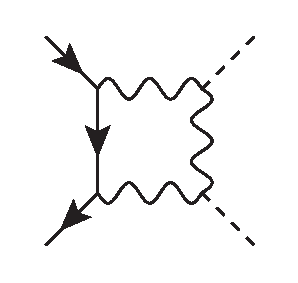
\includegraphics[height=0.10\textheight]{NLO_EW_SM/EW_qqbar_initiated/Images/VVVlo}}\label{fig:qqbarLO}}
	\qquad\qquad
    \subfloat[NLO virtual.]{{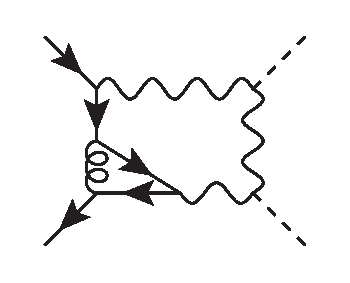
\includegraphics[height=0.10\textheight]{NLO_EW_SM/EW_qqbar_initiated/Images/VVVv}}\label{fig:qqbarV}}
	\qquad\qquad
    \subfloat[NLO real.]{{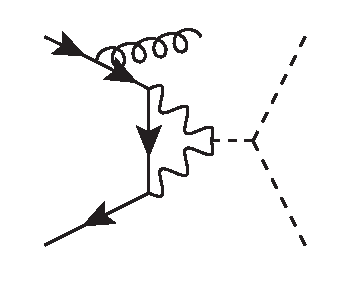
\includegraphics[height=0.10\textheight]{NLO_EW_SM/EW_qqbar_initiated/Images/HHHr}}\label{fig:qqbarR}}
	\qquad\quad

	\caption{Representative diagrams for light-quark-antiquark-initiated contributions from Ref.~\cite{Bonetti:2026cih}.}
    \label{fig:amplqqbar}
\end{figure}

\noindent The process $q\overline{q} \to hh$, mediated by weak bosons in the loop, has been calculated in Ref.~\cite{Bonetti:2026cih}, including NLO QCD corrections and considering only light quarks. Fig.~\ref{fig:amplqqbar} shows illustrative diagrams at LO and at NLO QCD. Only the first two generations of quarks are considered as initial states.

The $q\overline{q}hh$ two-loop diagrams and the $q\overline{q}hhg$ real emission diagrams contributing at NLO can be decomposed into subsets according to the number of $VVH$ or $VVhh$ vertices and vector boson propagators they contain, analogous to the light-quark contributions to $gg \to hh$ described in Section~\ref{EW:light-quark} and calculated in Ref.~\cite{Bonetti:2025vfd}.

For the two-loop virtual diagrams, only the $VVV$ subset (exemplified in Fig.~\ref{fig:amplqqbar}b) is non-zero, due to angular momentum conservation. Consequently, real emissions belonging to the $VVh$ and $VVhh$ blocks do not develop IR poles when integrating over the phase space of the unresolved extra gluon.

The one-loop amplitudes have been evaluated via the computer code \texttt{GoSam-3.0}~\cite{Braun:2025afl}, while the two-loop virtual contributions have been calculated analytically, retaining full dependence on the Mandelstam invariants and masses. The two-loop Feynman integrals have been reduced to master integrals, which have been expressed in terms of Chen iterated integrals over logarithmic kernels. Differential equations tailored to the independent transcendental functions at the level of the form factors have been constructed to produce precise numerical evaluations through the \texttt{Mathematica} package \texttt{DiffExp}~\cite{Hidding:2020ytt}.

The full set of NLO amplitudes has been implemented in the form of numerical grids in the {\tt POWHEG-BOX-V2} framework. NLO QCD corrections increase the total cross section with respect to LO $q\overline{q} \to hh$ by about $+60\%$.

On the one hand, the contribution to the total cross section coming from the quark-antiquark channel is negligible when compared to the gluon channel, amounting to about $+0.35\%$. On the other hand, the NLO QCD corrections to $q\overline{q} \to hh$ have a large shape-distorting effect at low energies in the $m_{hh}$ differential distribution, increasing the leftmost bin by about $10\%$ (cf.\ Fig.~\ref{fig:invariantMass}).\footnote{Bins with a $20\,\textup{GeV}$ width are considered.} As the low $m_{hh}$ region is also very sensitive to deviations of the trilinear Higgs boson self-coupling from the SM value, these contributions should not be neglected in high-precision predictions for Higgs boson pair production.


\begin{figure}
\centering
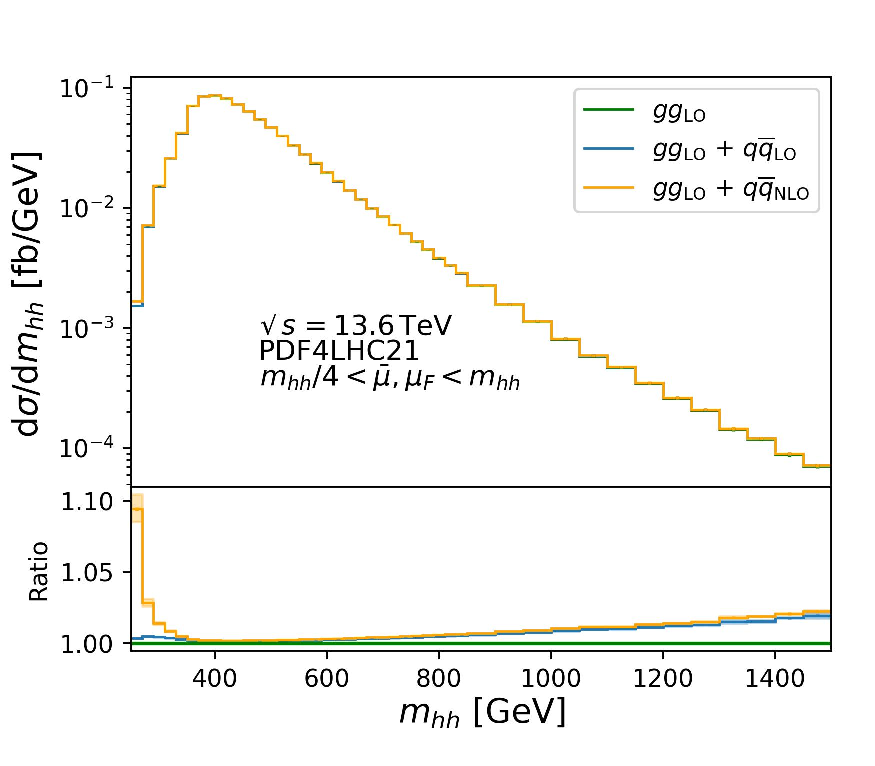
\includegraphics[width=0.49\textwidth]{NLO_EW_SM/EW_qqbar_initiated/Images/1a_HH-m_hfix.pdf}
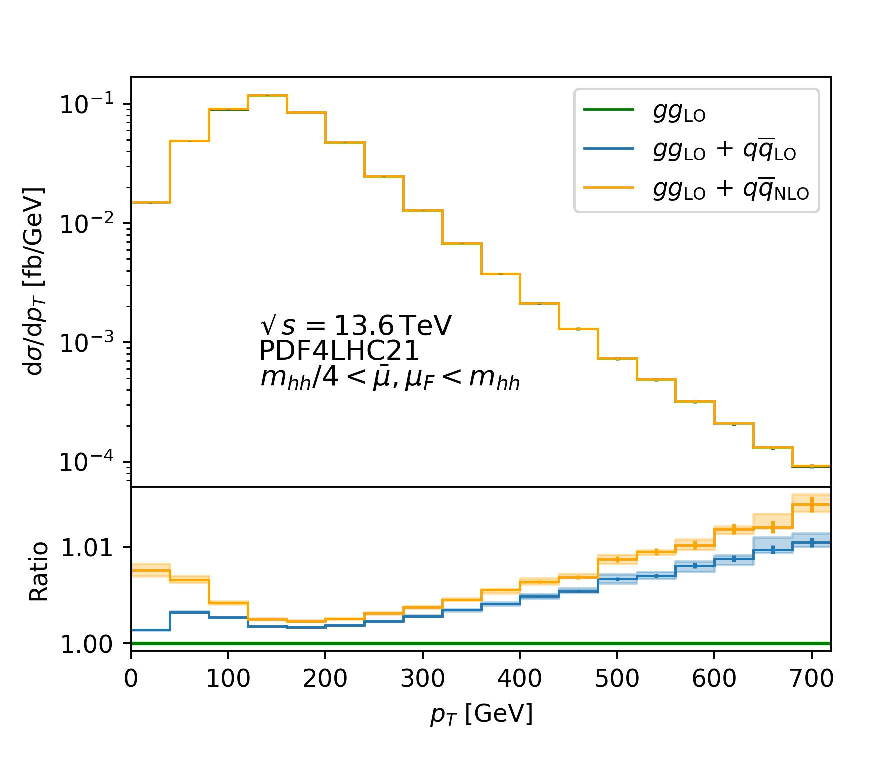
\includegraphics[width=0.49\textwidth]{NLO_EW_SM/EW_qqbar_initiated/Images/2a_H-pt_hfix.pdf}
\caption{Invariant mass distribution of the Higgs boson pair (left) and transverse momentum distribution (right) of a single Higgs boson at a proton-proton centre-of-mass energy of $\sqrt{s} = 13.6\,\textup{TeV}$. The error bands represent the scale uncertainties of the quark-antiquark channel and the error bars indicate the statistical uncertainties from the Monte Carlo integration. Figures from Ref.~\cite{Bonetti:2026cih}.
}
\label{fig:invariantMass}
\end{figure}
